% Chapter 12

\chapter{Interpretations} % Chapter title
\label{ch:interpretations} 

Using the simplified models discussed in \autoref{sec:simplified_models}, these results can be interpreted into exclusions of theories based on the masses of the particles involved. Of course, these exclusions include all the assumptions of the models used, so they shouldn't be interpreted to mean that no theory with a given set of particle masses can possibly exist, but they do provide a helpful guideline for targeting future searches and comparing results from different analyses.

Limits are determined using a program called HistFitter \cite{Baak:2014wma}, designed within the \ac{ATLAS} experiment, which builds upon the capabilities of ROOT \cite{BRUN199781}, RooStats \cite{1009.1003}, and HistFactory \cite{Cranmer:2012sba} to combine the uncertainties of the various background predictions, including their correlations, and produce cross-section limits at 95\% \ac{CL} using the $CL_{\text{S}}$ prescription~\cite{statforumlimits,clsread}. In this prescription, a likelihood is constructed based on the expected signal and background contributions to the \ac{SR}. Nuisance parameters are created based on the statistical and systematic uncertainties for each data-driven background, as well as for each systematic applied to the \ac{MC}-driven background estimates. The fit uses Gaussian models for nuisance parameters for all signal and background uncertainties, except for the statistical uncertainty on data- and \ac{MC}-driven background estimates, which are interpreted as Poissonian. Experimental uncertainties are considered fully correlated across the signal and background \ac{MC}-based estimates. 

A fit is performed, leaving a signal strength parameter ($\mu$) free, to maximize the likelihood, and subsequent fits are preformed to at discrete $\mu$ values to determine the relative likelihood of each value. Using this relative likelihood, the probability of a background-only hypothesis, $p_b$, can be determined by setting $\mu=0$, as well as the probability of a signal + background hypothesis $p_{s+b}$ with any non-zero signal strength, but nominally with $\mu=1$. The confidence limit is constructed as a ratio

\begin{equation}
CL_S = \frac{p_{s+b}}{1-p_b}. 
\end{equation}

Then, if $CL_S$ falls below 5\%, the signal + background hypothesis can be excluded at 95\%. Expected exclusion limits are constructed by assuming the observed data precisely matches the prediction, and 1$\sigma$ uncertainty bands are formed by varying the nuisance parameters away from their fitted values to produce a change in the likelihood. The observed limit uses the actual observation of data in the \ac{SR} to set exclusion limits, so any excess above the expected background will result in worse limits than expected, and any deficit will result in better limits. This exclusion is typically displayed with error bands that represent a 1$\sigma$ variation in the cross-section of the signal models. 

The simplified model discussed in \autoref{sec:simplified_models}, in which pair-produced gluinos decay via a $\chitwozero$ to jets, a $Z$ boson, and a $\chionezero$ \ac{LSP}, is produced in two grids, which differ by their choice of the \ac{LSP} mass. The first grid assumes a light \ac{LSP}, fixing its mass to 1 \gev~ for all mass points, and is shown as a function of $\tilde{g}$ and $\chitwozero$. The second grid is defined as a function of $\tilde{g}$ and $\chionezero$, and its varying \ac{LSP} mass is defined relative to the $\chitwozero$ mass by $m(\tilde{\chi}^{0}_{1}) = m(\tilde{\chi}^{0}_{2}) - 100 \gev$. \autoref{fig:excl_SMGGN2_1} shows the first of these grids, along with exclusions on a similar simplified model, which replaces the gluinos with squarks and uses the same mass scheme. The exclusion contours on the second grid is shown in \autoref{fig:excl_SMGGN2}, as a function of $m(\tilde{g})$ and $m(\tilde{\chi}^{0}_{1})$.

\begin{figure}[!htb]
\centering
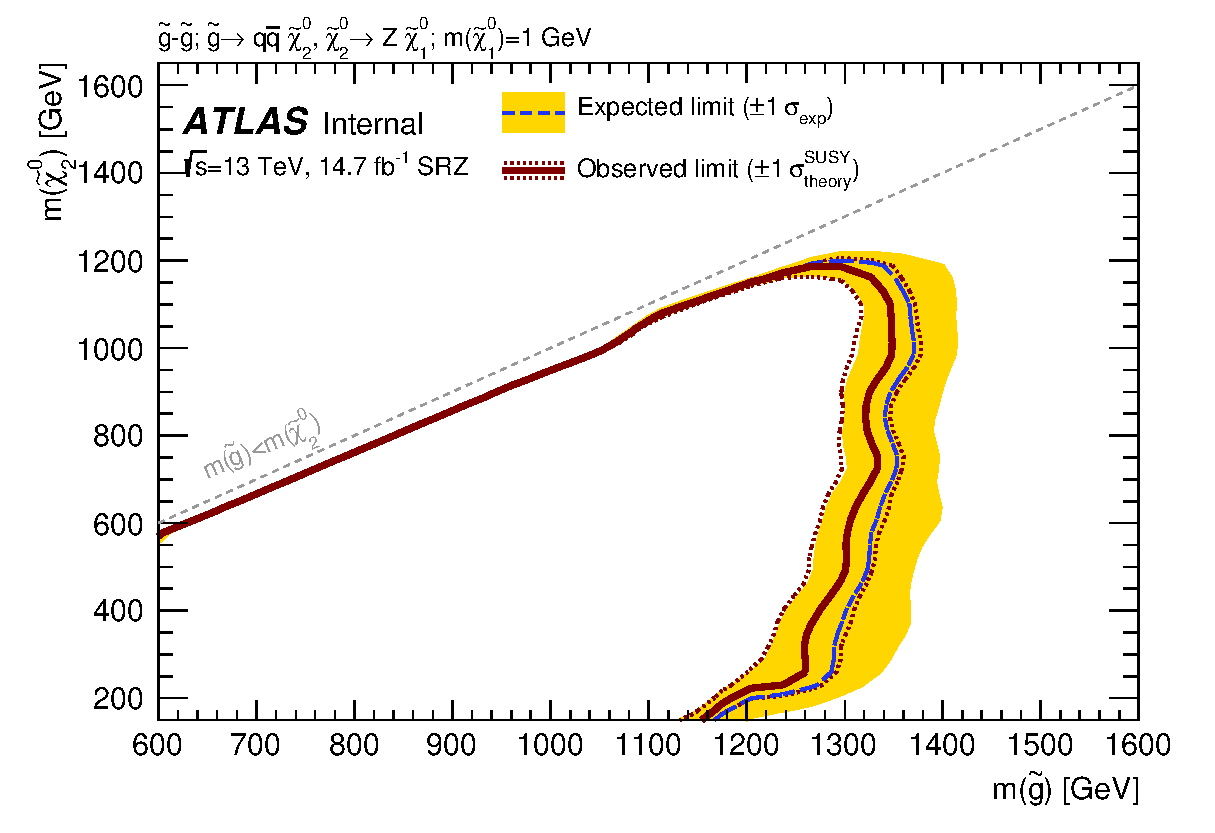
\includegraphics[width=.8\textwidth]{figures/interpretation/excl_SM_GG_N2_1.eps}
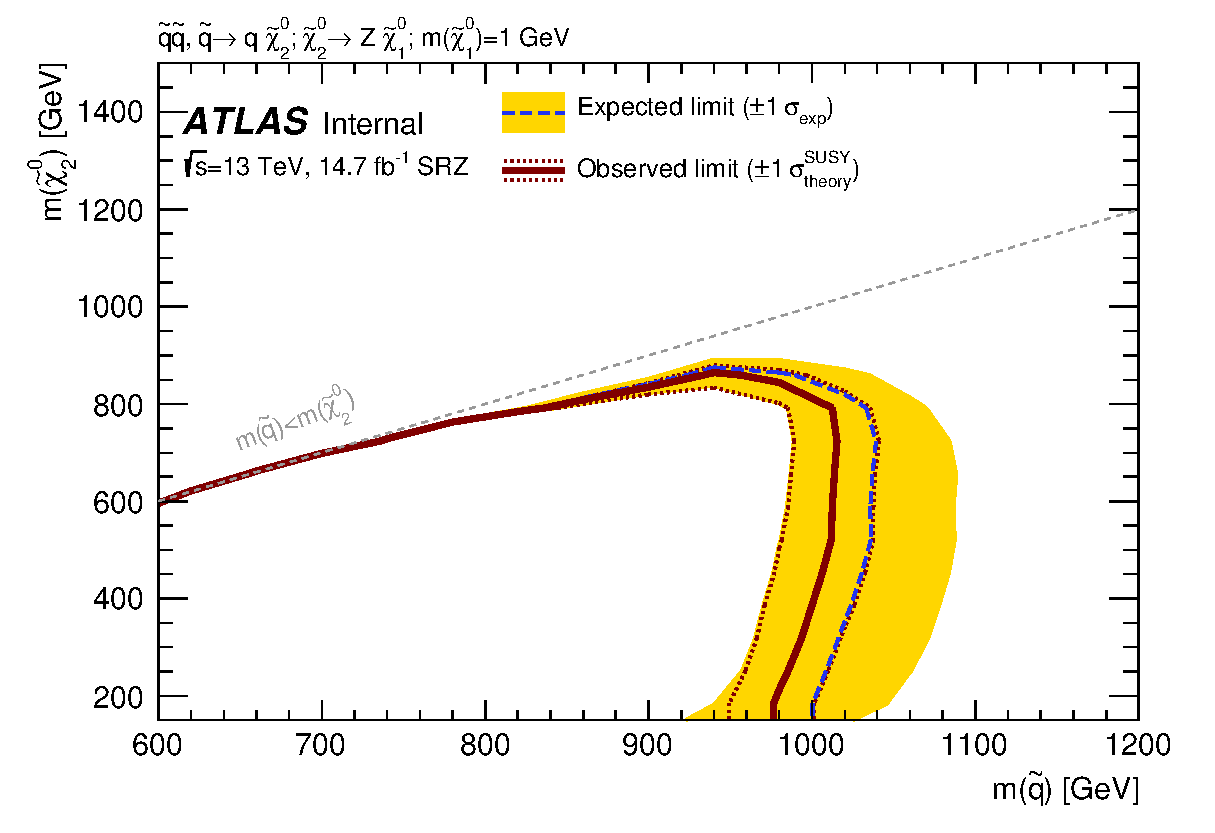
\includegraphics[width=.8\textwidth]{figures/interpretation/excl_SM_SS_N2.eps}  
\caption{
Expected and observed exclusion contours derived from the results in SRZ for the (top) $\tilde{g}$--$\chitwozero$ on-shell grid and (bottom) $\tilde{q}$--$\chitwozero$ on-shell grid. 
The dashed blue line indicates the expected limits at $95\%$ CL and the yellow band shows the $1\sigma$ variation of the expected limit as a consequence of the uncertainties in the background prediction and the experimental uncertainties in the signal ($\pm1\sigma_\text{exp}$). 
The observed limits are shown by the solid red line, with the dotted red lines indicating the variation resulting from changing the signal cross section within its uncertainty ($\pm1\sigma^\text{SUSY}_\text{theory}$). \label{fig:excl_SMGGN2_1}
}
\end{figure}

\begin{figure}[!htb]
\centering
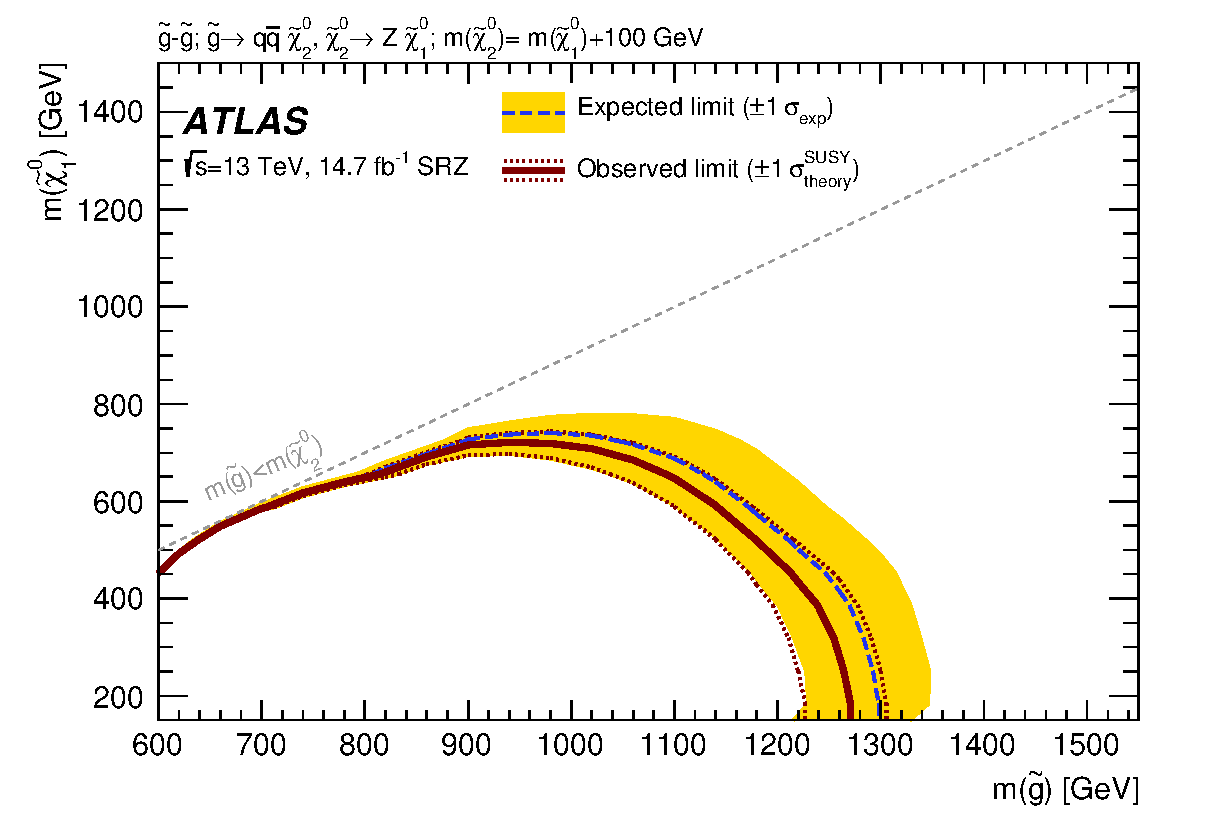
\includegraphics[width=.8\textwidth]{figures/interpretation/excl_SM_GG_N2.eps}
\caption{
Expected and observed exclusion contours derived from the results in SRZ for the $\tilde{g}$--$\chionezero$ on-shell grid. 
The dashed blue line indicates the expected limits at $95\%$ CL and the yellow band shows the $1\sigma$ variation of the expected limit as a consequence of the uncertainties in the background prediction and the experimental uncertainties in the signal ($\pm1\sigma_\text{exp}$). 
The observed limits are shown by the solid red line, with the dotted red lines indicating the variation resulting from changing the signal cross section within its uncertainty ($\pm1\sigma^\text{SUSY}_\text{theory}$).
\label{fig:excl_SMGGN2}
}
\end{figure}

In general, the observed exclusions are slightly weaker than the expected exclusions, due to a very small excess of events observed in SRZ. The observed lower limit on $m(\tilde{g})$ is about 1.3 \tev~for models with $m(\tilde{\chi}^{0}_{2})$ = 500 \gev~for the $\tilde{g}$--$\chitwozero$ grid. These improve significantly on the previous \ac{ATLAS} exclusion, which used different models for interpretation, but placed a lower limit on $m(\tilde{g})$ at around 900 \gev~for similar $m(\tilde{\chi}^{0}_{2})$. 



%----------------------------------------------------------------------------------------
